\section{Related Approaches}
\begin{frame}{Related Approaches}
  \begin{itemize}
    \item Optimizing black-box problems
      \begin{itemize}
        \item No deterministic way to evolve global optimum.
        \item Applying random search for approximation.
      \end{itemize}
      \vspace*{14pt}
    \item Stochastic algorithms
      \begin{itemize}
        \item Ant Colony Optimization, Bat Algorithm, etc.
        \item Iteratively generating better solutions.
      \end{itemize}
      \vspace*{14pt}
    \item Two major approaches
      \begin{itemize}
        \item Estimation of distribution algorithm (EDA).
        \item Evolution strategy (ES).
      \end{itemize}
  \end{itemize}
\end{frame}

\subsection{Real-coded Extended Compact Genetic Algorithm}

\begin{frame}{EDA}
  \begin{itemize}
    \item Also known as Probabilistic Model Building GA (PMBGA).\pause
      \begin{itemize}
        \item Building model explicitly.
        \item Linkage between decision variables are provided.\pause
      \end{itemize}
      \vspace*{14pt}
    \item Mechanism difference with traditional GA.
      \begin{itemize}
        \item Operators `crossover' and `mutation' are replaced with
          `modeling' and `sampling'.        \pause
          \begin{figure}
            \centering
            \only<4>{\includegraphics[height = 0.5\textheight]{EDA.eps}}
          \end{figure}
      \end{itemize}
  \end{itemize}
\end{frame}

\begin{frame}{Extended Compact Genetic Algorithm (ECGA)}
  \begin{itemize}
    \item Each EDA is different from the others in \alert{model
      building}.
      \vspace*{14pt}
    \item ECGA was proposed by Harik (1999).
      \vspace*{14pt}
    \item Good probabilistic model inspires good linkage learing
      \begin{itemize}
        \item Model is built according to population distribution.
        \item Applying greedy search to refine model iteratively.
      \end{itemize}
      \vspace*{14pt}
    \item ECGA focuses on bitstring, discrete problems.
      \begin{itemize}
        \item $\chi$-ECGA.
        \item An interface for real-valued function is demanded.
      \end{itemize}
  \end{itemize}
\end{frame}

\begin{frame}{Discretization} 
  \begin{itemize} 
    \item Continuous domain $\rightarrow$ Discrete domain 
    \item Finding good solutions $\rightarrow$ Finding promising
      regions
    \item 2 traditional discretization methods
      \begin{itemize}
        \item Fixed Height Histogram (FHH)
        \item Fixed Width Histogram (FWH)
      \end{itemize}
  \end{itemize}
  \begin{minipage}{.45\textwidth}
    \begin{figure}
      \centering
      \includegraphics[width =0.6\linewidth]{FHH.eps}
      \caption{illustration of FHH}
    \end{figure}
  \end{minipage}
  \begin{minipage}{.45\textwidth}
    \begin{figure}
      \centering
      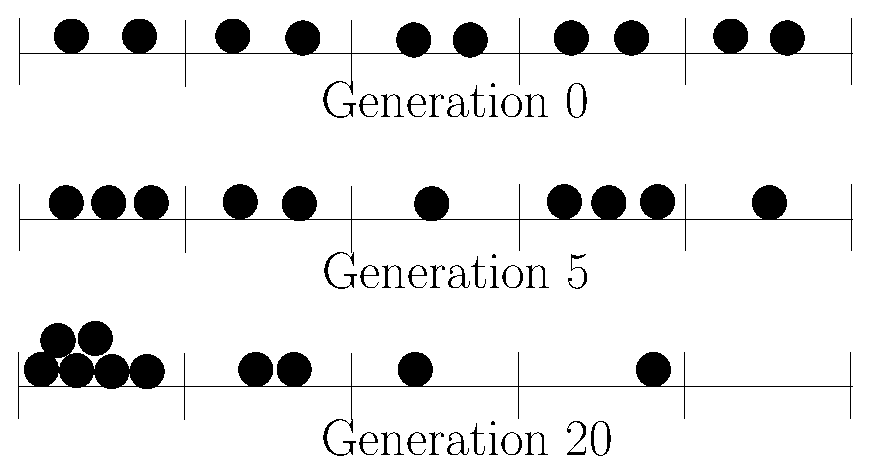
\includegraphics[width =0.7\linewidth]{FWH.eps}
      \caption{illustration of FWH}
    \end{figure}
  \end{minipage}

\end{frame}

\begin{frame}{Split on Demand}
  \begin{itemize}
    \item Solutions in each bin should not exceed $\gamma N$.
      \begin{itemize}
        \item $N$ is the population size.
        \item $\gamma$ defines the rate of one region.
      \end{itemize}
    \item $\gamma$ decays with a factor $\epsilon$.
  \end{itemize}
  \begin{figure}
    \centering
    \includegraphics[scale = 0.3]{SoD.eps}
    \caption{illustration of SoD}
  \end{figure}
\end{frame}

\begin{frame}{Real-coded ECGA with SoD}
  \pause
  \begin{enumerate}
    \item Preparing discretization\pause
      \vspace*{14pt}
    \item Integrating discretized results into ECGA.\pause
      \vspace*{14pt}
    \item ECGA builds model accordingly, output the promising
      regions.\pause
      \vspace*{14pt}
    \item Sampling accordingly.\pause
      \vspace*{14pt}
    \item For every $L$ generations, a local optimizer is adopted to
      obtain high resolution solutions\pause
      \vspace*{14pt}
    \item If model does not converge, goto 1.
  \end{enumerate}
\end{frame}

\subsection{Covariance Matrix Adaptation Evolution Strategy}


\begin{frame}{Evolution Strategy (ES)}
  \begin{itemize}
    \item A search template for black-box optimization.
      \begin{itemize}
        \item Encoded in continuous domain.
      \end{itemize}
      \vspace*{14pt}
    \item New search points are generated based on current population.
      \vspace*{14pt}
    \item $(\mu,\lambda)$-ES and $(\mu,\mu+\lambda)$-ES.
      \vspace*{14pt}
    \item $x_i^{t+1} = m^t + \sigma N_i(0,C)$.
      \begin{itemize}
        \item $x_i$: $i$-th generated solution at generation $t+1$.
        \item $m$: weighted mean of population at generation $t$.
        \item $\sigma$: step size.
        \item $C$: Estimated distribution.
      \end{itemize}
  \end{itemize}
\end{frame}

\begin{frame}{Covariance Matrix Adaptation Evolution Strategy (CMA-ES)}
  \begin{itemize}
    \item A famous derivation of ES.
      \vspace*{14pt}
    \item Importance of $\sigma$ and $C$.
      \begin{itemize}
        \item Larger step size reinforces exploration while smaller
          reinforces exploitation.
          \begin{itemize}
            \item Choosing an fixed, appropriate number?
          \end{itemize}
        \item Covariance matrix determines the shape of estimated
          distribution.
          \begin{itemize}
            \item Determining the length of each axis.
            \item Representing the dependency among decision variables.
          \end{itemize}
      \end{itemize}
          \vspace*{14pt}
        \item CMA-ES features in the adoption of historical information.
          \begin{itemize}
            \item $\sigma$ and $C$ are adjusted accordingly.
          \end{itemize}
  \end{itemize}
\end{frame}

\begin{frame}{Illustration of $\sigma$ and $C$}
  \begin{columns}
    \begin{column}{.33\textwidth}
      \begin{figure}
        \centering
        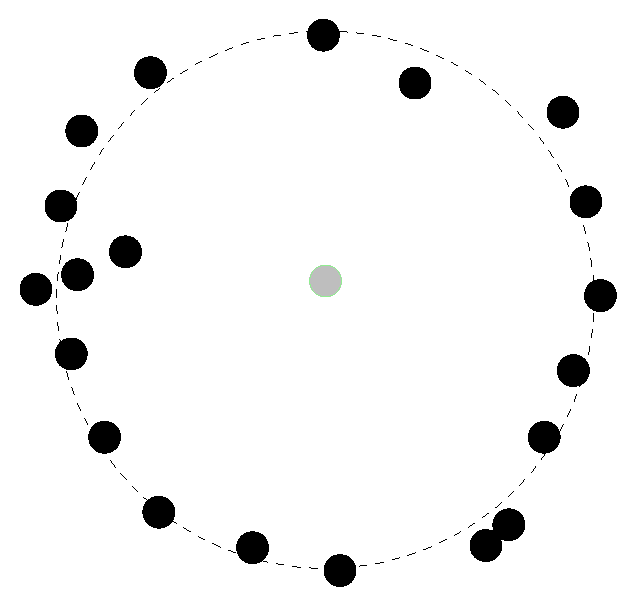
\includegraphics[width=.9\textwidth]{ES_0.eps}
        \caption{$t$ = 0}
      \end{figure}
    \end{column}
    \begin{column}{.33\textwidth}
      \begin{figure}
        \centering
        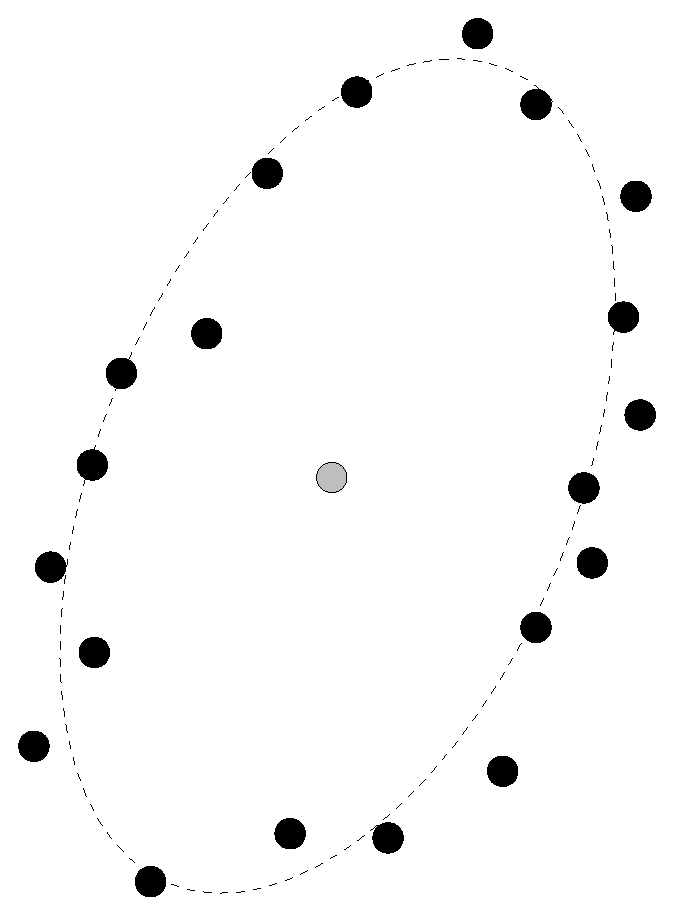
\includegraphics[width=.9\textwidth]{ES_10.eps}
        \caption{$t$ = 10}
      \end{figure}
    \end{column}
    \begin{column}{.33\textwidth}
      \begin{figure}
        \centering
        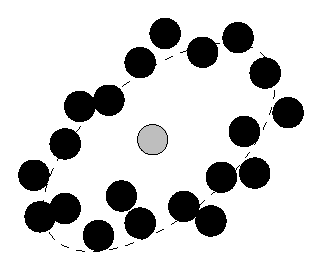
\includegraphics[width = .9\textwidth]{ES_20.eps}
        \caption{$t$ = 20}
      \end{figure}
    \end{column}
  \end{columns}
\end{frame}

